\documentclass[11pt]{article}
\usepackage[a4paper, margin=2.5cm]{geometry}
\usepackage{graphicx}
\usepackage{caption}
\usepackage{pdfcomment}
\usepackage{float}
\usepackage{tikz}
\captionsetup{font=small, skip=6pt}
\usepackage{titlesec}
\usepackage{parskip}
\setlength{\parskip}{4pt}
\setlength{\textfloatsep}{10pt}
\setlength{\floatsep}{6pt}
\setlength{\intextsep}{10pt}

\titlespacing*{\section}{0pt}{2ex plus .2ex minus .2ex}{1ex plus .2ex}
\titlespacing*{\subsection}{0pt}{1ex plus .1ex minus .1ex}{0.5ex plus .1ex}


\usepackage{parskip}
\setlength{\parskip}{2pt}

\title{Wzmacniacze mocy w napędzie elektrycznym. Przekształtnik tranzystorowy i tyrystorowy.}

\author{
  Mateusz Jaworski \\
  Piotr Migdalek \\
  Pawel Michalski \\
  Jakub Jaszczak \\
  Franciszek Janicki
}

\begin{document}

\maketitle

\section{Część I}

\subsection{WZMACNIACZ LINIOWY / WZMACNIACZ IMPULSOWY}

a) Badanie sprawnosci wzmacniacza liniowego BJT

\begin{figure}[H]
\centering
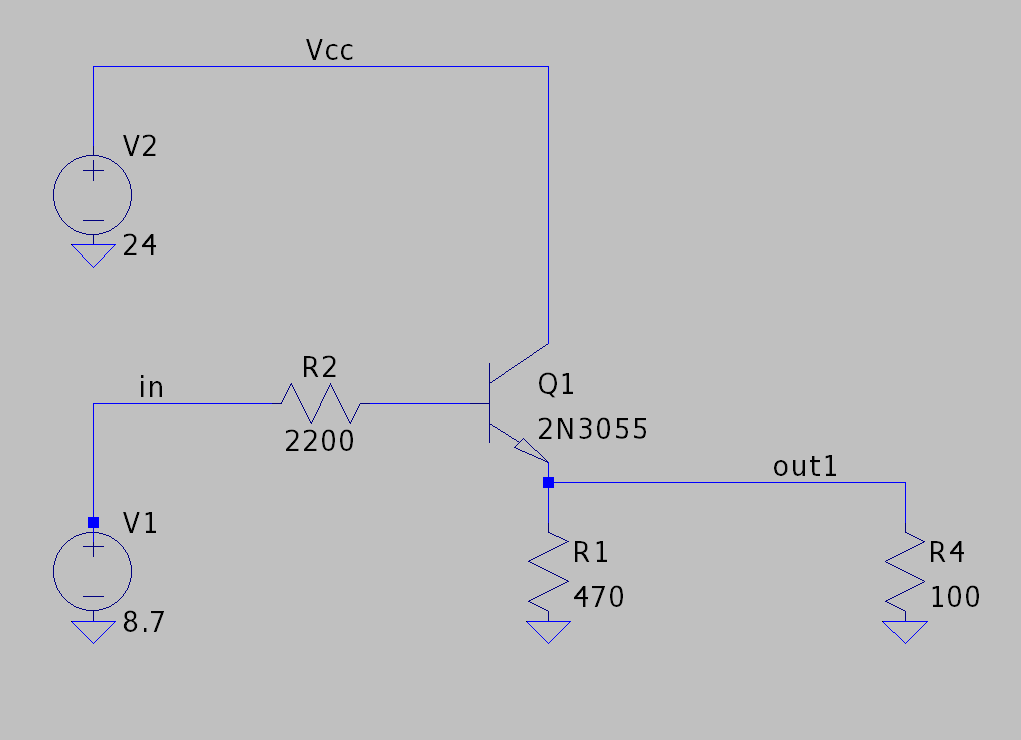
\includegraphics[width=0.8\textwidth]{aun1_liniowy_bjt.png}
\caption{Schemat pomiarowy wzmacniacza liniowego BJT}
\end{figure}

\begin{table}[H]
\centering
\begin{tabular}{|c|c|c|c|c|}
\hline
\textbf{Vcc [V]} & \textbf{V\_in [V]} & \textbf{P\_in + P\_vcc [mW]} & \textbf{P\_out [W]} & \textbf{Sprawność [\%]} \\
\hline
24 & 2  & 0{,}667  & 0{,}014683 & 2{,}201 \\
\hline
24 & 4  & 1{,}525  & 0{,}070000 & 4{,}590 \\
\hline
24 & 6  & 2{,}380  & 0{,}166000 & 6{,}975 \\
\hline
24 & 8  & 3{,}242  & 0{,}360000 & 11{,}104 \\
\hline
24 & 10 & 4{,}097  & 0{,}477000 & 11{,}643 \\
\hline
24 & 12 & 4{,}950  & 0{,}690000 & 13{,}939 \\
\hline
24 & 14 & 5{,}800  & 0{,}941000 & 16{,}224 \\
\hline
24 & 16 & 6{,}640  & 1{,}220000 & 18{,}373 \\
\hline
24 & 18 & 7{,}490  & 1{,}540000 & 20{,}561 \\
\hline
24 & 20 & 8{,}330  & 1{,}940000 & 23{,}289 \\
\hline
\end{tabular}
\caption{Sprawnosc pracy wzmacniacza liniowego BJT}
\end{table}

b) Badanie sprawnosci wzmacniacza impulsowego BJT, porownanie z wzmacniaczem liniowym BJT

\begin{figure}[H]
\centering
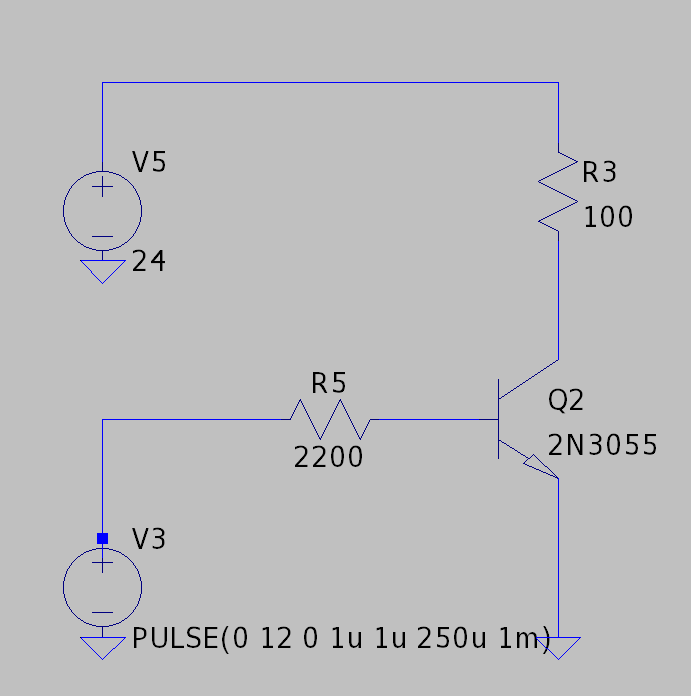
\includegraphics[width=0.8\textwidth]{aun1_impulsowy_bjt.png}
\caption{Schemat pomiarowy wzmacniacza impulsowego BJT}
\end{figure}

\begin{table}[H]
\centering
\begin{tabular}{|c|c|c|c|c|}
\hline
\textbf{Vcc [V]} & \textbf{V\_in [V]} & \textbf{P\_vcc + P\_in [W]} & \textbf{P\_out [W]} & \textbf{Sprawność [\%]} \\
\hline
24 & 2  & 0{,}54825 & 0{,}499   & 91{,}017 \\
\hline
24 & 4  & 1{,}054   & 0{,}974   & 92{,}410 \\
\hline
24 & 6  & 1{,}549   & 1{,}453   & 93{,}802 \\
\hline
24 & 8  & 2{,}046   & 1{,}928   & 94{,}233 \\
\hline
24 & 10 & 2{,}544   & 2{,}4023  & 94{,}430 \\
\hline
24 & 12 & 3{,}0476  & 2{,}882   & 94{,}566 \\
\hline
24 & 14 & 3{,}545   & 3{,}356   & 94{,}669 \\
\hline
24 & 16 & 4{,}042   & 3{,}831   & 94{,}780 \\
\hline
24 & 18 & 4{,}546   & 4{,}311   & 94{,}831 \\
\hline
24 & 20 & 5{,}043   & 4{,}833   & 95{,}836 \\
\hline
\end{tabular}
\caption{Sprawnosc pracy wzmacniacza impulsowego BJT}
\end{table}

\begin{figure}[H]
\centering
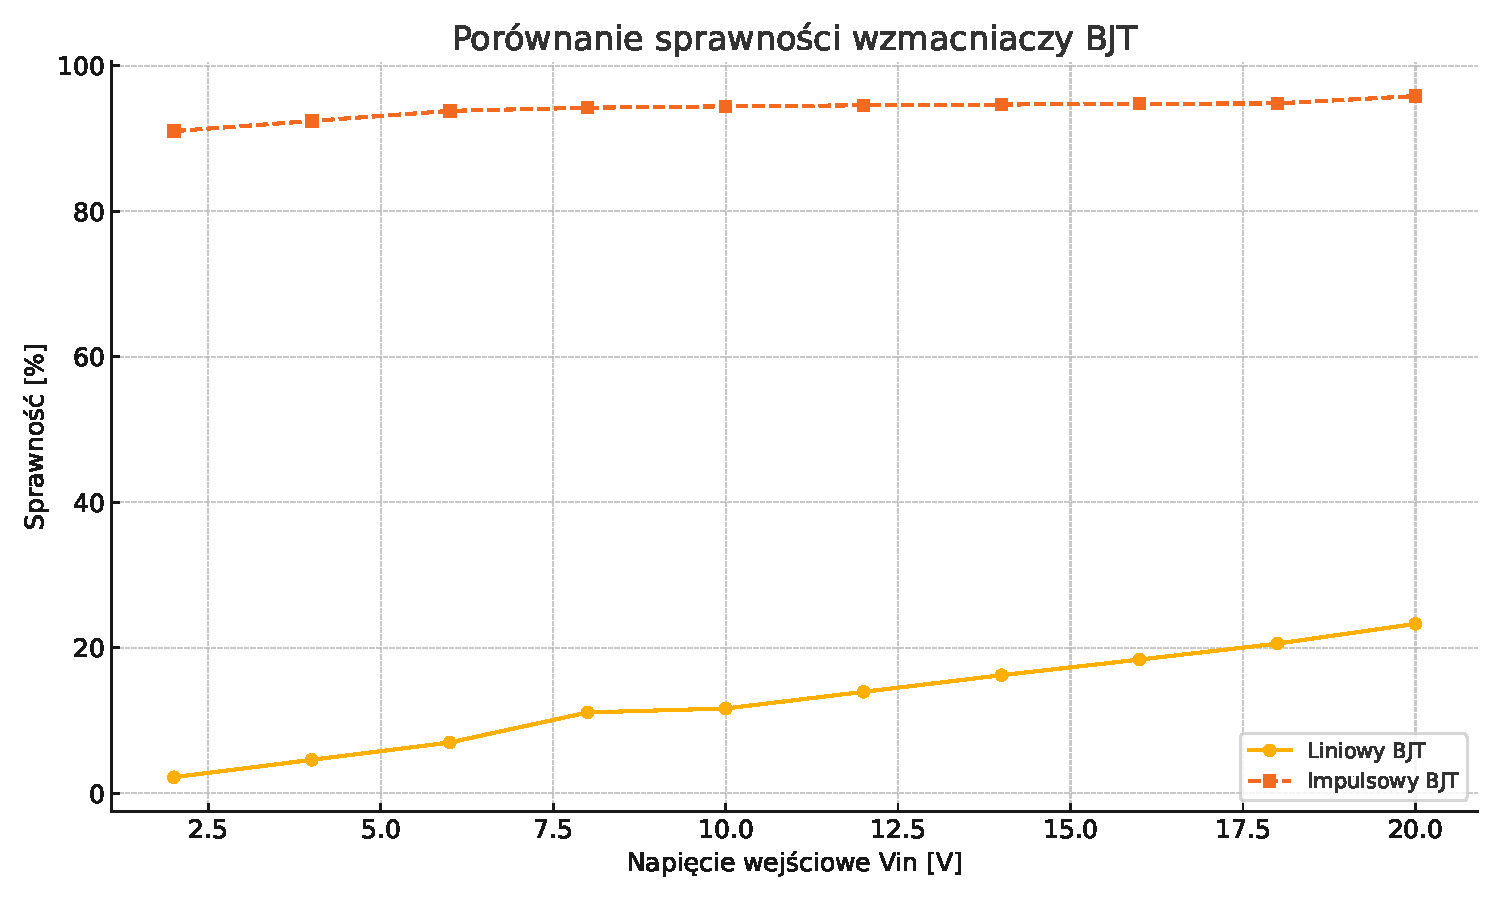
\includegraphics[width=0.8\textwidth]{aun1_liniowy_impulsowy_bjt.pdf}
\caption{Wykres sprawnosci wzmacniacza liniowego i impulsowego BJT}
\end{figure}

\subsection{TECHNOLOGIA BJT/MOSFET}

c) Badanie sprawności wzmacniacza impulsowego MOSFET i porównanie z wzmacniaczem impulsowym BJT oraz porównanie wpływu Rds_on i ładunku bramki na sprawność

\begin{figure}[H]
\centering
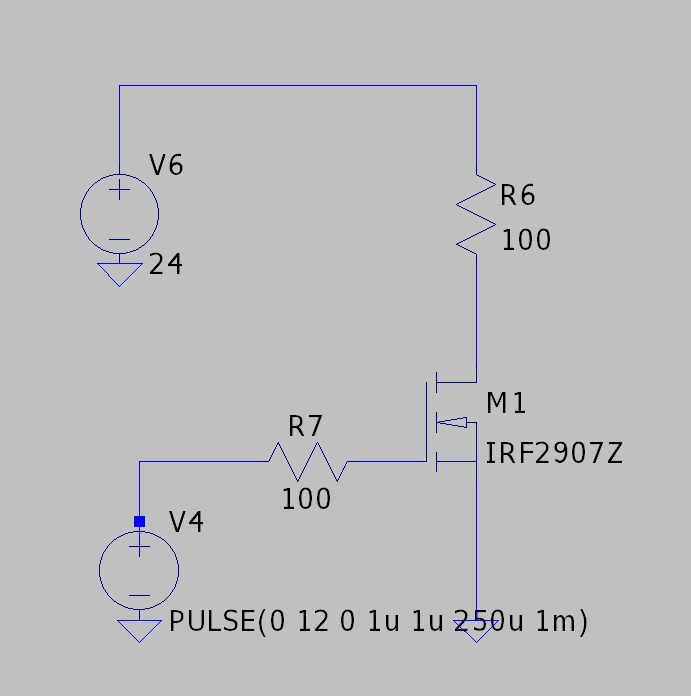
\includegraphics[width=0.8\textwidth]{aun1_impulsowy_mosfet.png}
\caption{Schemat pomiarowy wzmacniacza impulsowego MOSFET}
\end{figure}

\begin{table}[H]
\centering
\begin{tabular}{|c|c|c|c|c|}
\hline
\textbf{Vcc [V]} & \textbf{V\_in [V]} & \textbf{P\_vcc + P\_in [mW]} & \textbf{P\_out [W]} & \textbf{Sprawność [\%]} \\
\hline
24 & 2  & 0{,}499    & 0{,}4956   & 99{,}319 \\
\hline
24 & 4  & 0{,}95412  & 0{,}9506   & 99{,}631 \\
\hline
24 & 6  & 1{,}461    & 1{,}4575   & 99{,}760 \\
\hline
24 & 8  & 1{,}939    & 1{,}9355   & 99{,}819 \\
\hline
24 & 10 & 2{,}417    & 2{,}4135   & 99{,}855 \\
\hline
24 & 12 & 2{,}9009   & 2{,}8974   & 99{,}879 \\
\hline
24 & 14 & 3{,}379    & 3{,}375    & 99{,}882 \\
\hline
24 & 16 & 3{,}857    & 3{,}853    & 99{,}896 \\
\hline
24 & 18 & 4{,}3409   & 4{,}3373   & 99{,}917 \\
\hline
24 & 20 & 5{,}760    & 5{,}759    & 99{,}983 \\
\hline
\end{tabular}
\caption{Sprawnosc pracy wzmacniacza impulsowego MOSFET}
\end{table}

\begin{figure}[H]
\centering
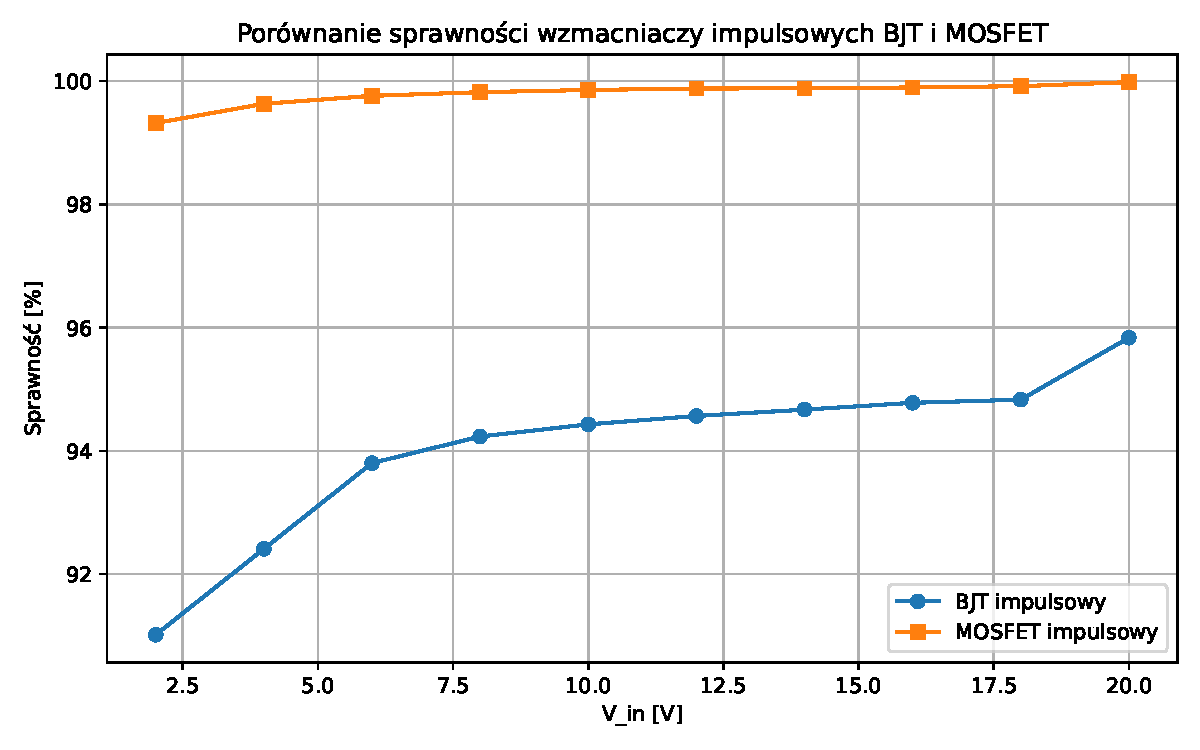
\includegraphics[width=0.8\textwidth]{aun1_imp_bjt_vs_mosfet.pdf}
\caption{Wykres sprawnosci wzmacniacza impulsowego BJT i MOSFET}
\end{figure}

\begin{table}[H]
\centering
\begin{tabular}{|c|c|c|}
\hline
\textbf{Parametr} & \textbf{IRFL4310} & \textbf{IRF2907Z} \\
\hline
Rds\_on & 200\,m\(\Omega\) & 3,5\,m\(\Omega\) \\
\hline
GateCharge & 28\,nC & 180\,nC \\
\hline
\end{tabular}

\caption{Porównanie parametrów tranzystorów IRFL4310 i IRF2907Z}
\end{table}

\begin{table}[H]
\centering
\begin{tabular}{|c|c|c|c|c|c|c|}
\hline
\textbf{f [Hz]} & \multicolumn{3}{c|}{\textbf{IRFL4310}} & \multicolumn{3}{c|}{\textbf{IRF2907Z}} \\
\cline{2-7}
 & $P_{in}+P_{vcc}$ [W] & $P_{out}$ [W] & Sprawność [\%] & $P_{in}+P_{vcc}$ [W] & $P_{out}$ [W] & Sprawność [\%] \\
\hline
1k   & 2,9009 & 2,8836 & 99,41 & 2,9009 & 2,8988 & 99,93 \\
\hline
2k   & 2,8917 & 2,8916 & 99,99 & 2,9219 & 2,9177 & 99,85 \\
\hline
4k   & 2,9078 & 2,9076 & 99,99 & 2,9638 & 2,9555 & 99,72 \\
\hline
8k   & 2,9400 & 2,9397 & 99,96 & 3,0478 & 3,0312 & 99,45 \\
\hline
16k  & 3,1335 & 3,1321 & 99,96 & --- & -- & --- \\
\hline
32k  & 3,1332 & 3,1319 & 99,92 & --- & --- & --- \\
\hline
64k  & 3,3909 & 3,3882 & 99,92 & --- & --- & --- \\
\hline
\end{tabular}
\caption{Porównanie sprawności tranzystorów IRFL4310 oraz IRF2907Z przy 50\% duty cycle. Dla częstotliwości PWM powyżej 64 kHz tranzystor IRFL4310 zaczyna nie nadążać z domykaniem oraz otwieraniem, natomiast dla częstotliwości 16 kHz robi to IRF2907Z.}
\end{table}

\begin{figure}[H]
\centering
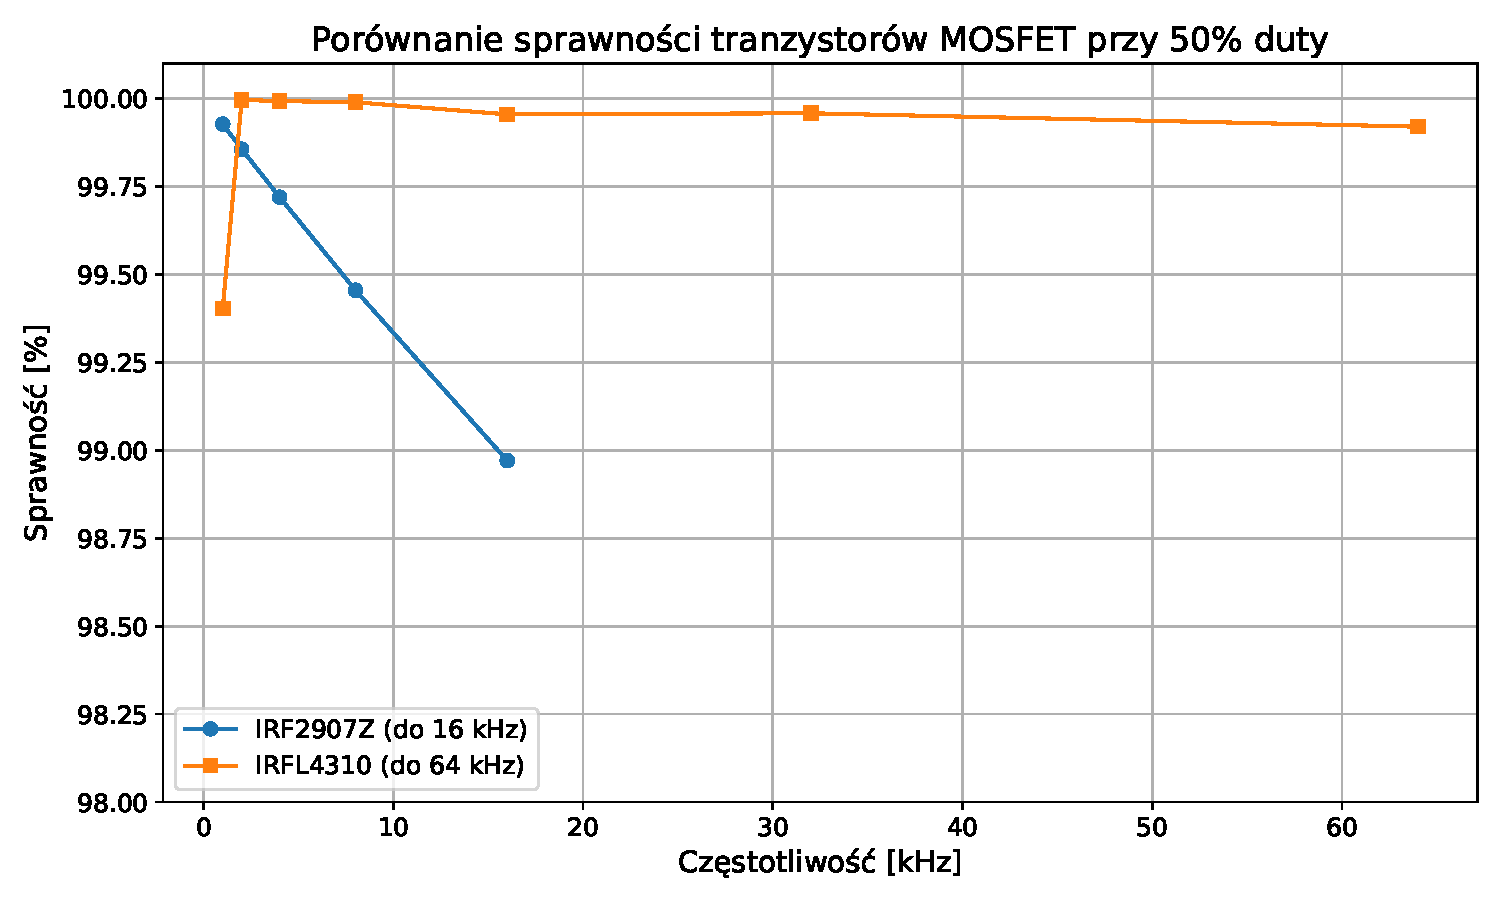
\includegraphics[width=0.8\textwidth]{aun1_imp_mosfet_comparison.pdf}
\caption{Wykres sprawnosci wzmacniaczy impulsowych MOSFET}
\end{figure}

\subsection{ZJAWISKA W OBWODZIE D-S TRANZYSTORA WYNIKAJĄCE Z PARAMETRÓW PASOŻYTNICZYCH OBWODU}

d) Badanie wartosci pasozytniczych w ukladzie RLD sterowanym tranzystorem MOSFET

\begin{figure}[H]
\centering
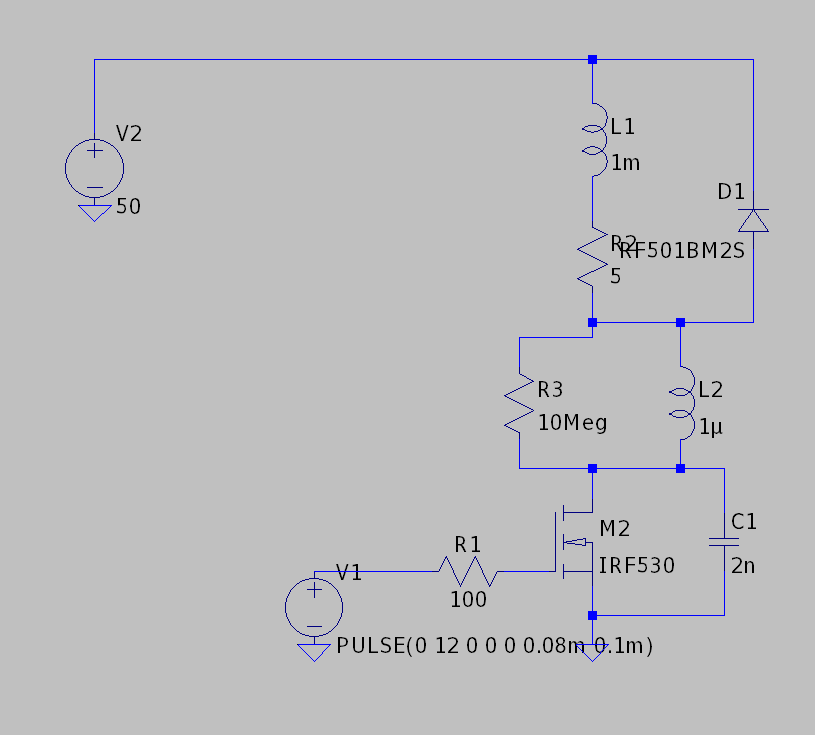
\includegraphics[width=0.8\textwidth]{aun1_rld_without_snubber.png}
\caption{Schemat pomiarowy ukladu RLD sterowanego tranzystorem MOSFET}
\end{figure}

\begin{figure}[H]
\centering
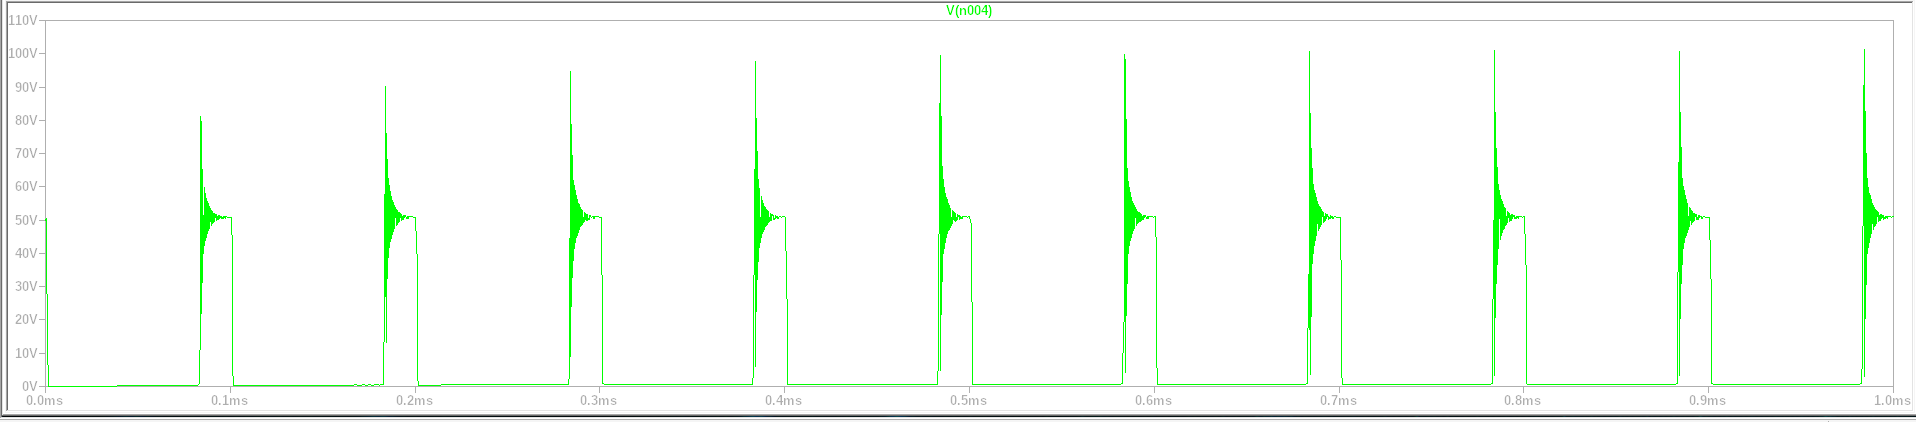
\includegraphics[width=0.8\textwidth]{aun1_rld_without_snubber_rgate100ohm.png}
\caption{Przebieg napiecia na wyjsciu tranzystora MOSFET sterujacego ukladem RLD z rezystancja bramki 100 [Ohm]}
\end{figure}

\begin{figure}[H]
\centering
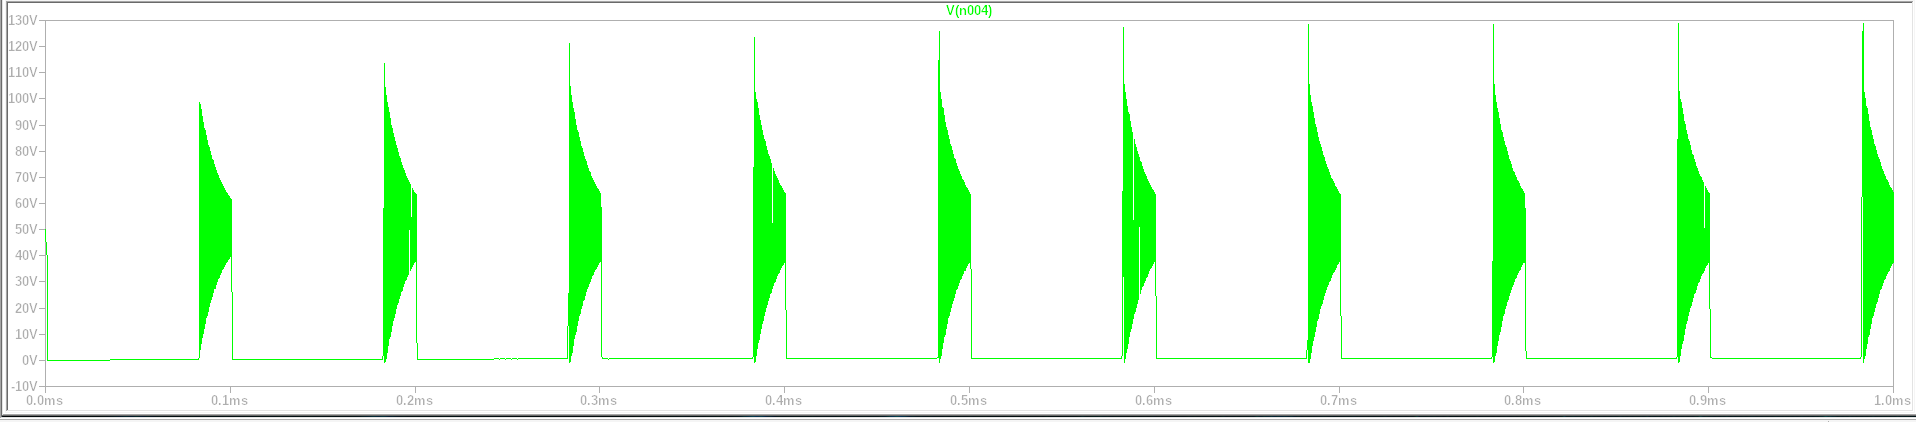
\includegraphics[width=0.8\textwidth]{aun1_rld_without_snubber_rgate10ohm.png}
\caption{Przebieg napiecia na wyjsciu tranzystora MOSFET sterujacego ukladem RLD z rezystancja bramki 10 [Ohm]}
\end{figure}

e) Dobor tlumika oscylacji napiecia (parametry snubber'a)

\begin{figure}[H]
\centering
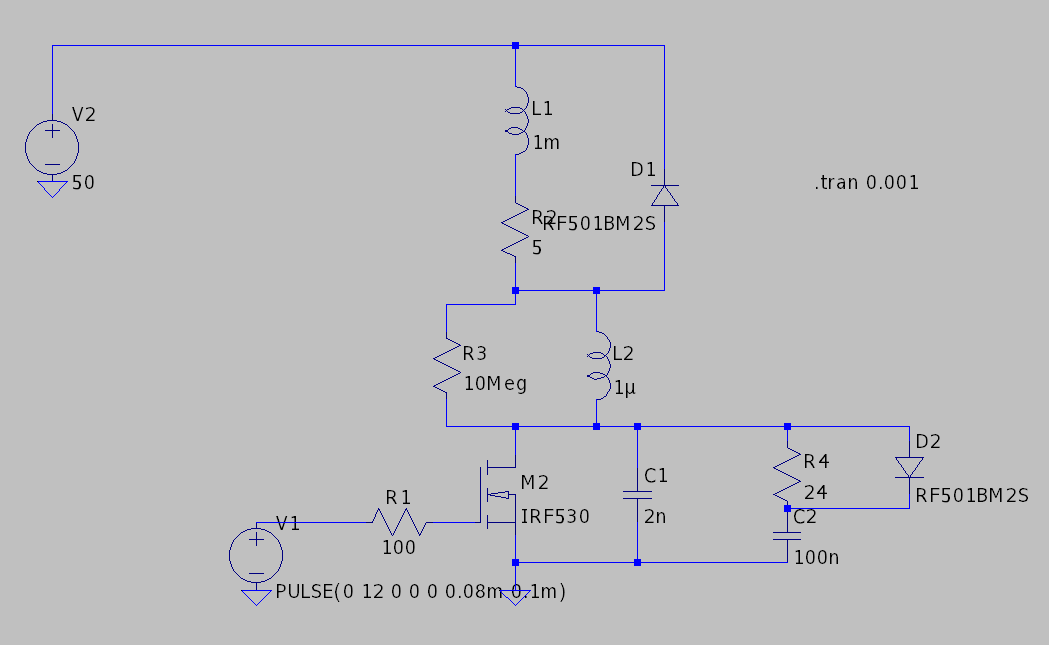
\includegraphics[width=0.8\textwidth]{aun1_rld_with_snubber.png}
\caption{Schemat pomiarowy ukladu RLD sterowanego tranzystorem MOSFET z tlumikiem oscylacji w obwodzie D-S tranzystora}
\end{figure}

Dobór parametrów tłumika (snubbera):
\begin{enumerate}
  \item Mierzymy częstotliwość oscylacji:
  \[
  f_0 = \SI{3.3}{\mega\hertz}
  \]
  \item Dobieramy kondensator o pojemności większej niż pojemność pasożytnicza tranzystora i mierzymy nową częstotliwość zakłóceń:
  \[
  C_1 = \SI{1}{\nano\farad}, \quad f_1 = \SI{2.7}{\mega\hertz}
  \]
  \item Liczymy stosunek częstotliwości:
  \[
  m = \frac{f_0}{f_1} = \frac{3.3}{2.7} = 1.22
  \]
  \item Obliczamy pojemność pasożytniczą tranzystora:
  \[
  C_0 = \frac{C_1}{m^2 - 1} = \frac{1\,\text{nF}}{1.22^2 - 1} = \SI{2.02}{\nano\farad}
  \]
  \item Obliczamy wartość indukcyjności pasożytniczej:
  \[
  L_0 = \frac{(m^2 - 1)}{(2\pi f_0)^2 C_1} = \frac{(1.22^2 - 1)}{(2\pi \cdot 3.3 \times 10^6)^2 \cdot 1 \times 10^{-9}} = \SI{1.15}{\micro\henry}
  \]
  \item Obliczamy minimalną wartość pojemności kondensatora snubbera:
  \[
  C_{\text{snubber}} = 3C_0 = 3 \cdot \SI{2.02}{\nano\farad} = \SI{6.06}{\nano\farad}
  \]
  \item Obliczamy wartość rezystancji w snubberze:
  \[
  R_{\text{snubber}} = \sqrt{\frac{L_0}{C_0}} = \sqrt{\frac{1.15 \times 10^{-6}}{2.02 \times 10^{-9}}} = \SI{24}{\ohm}
  \]
\end{enumerate}

\begin{figure}[H]
\centering
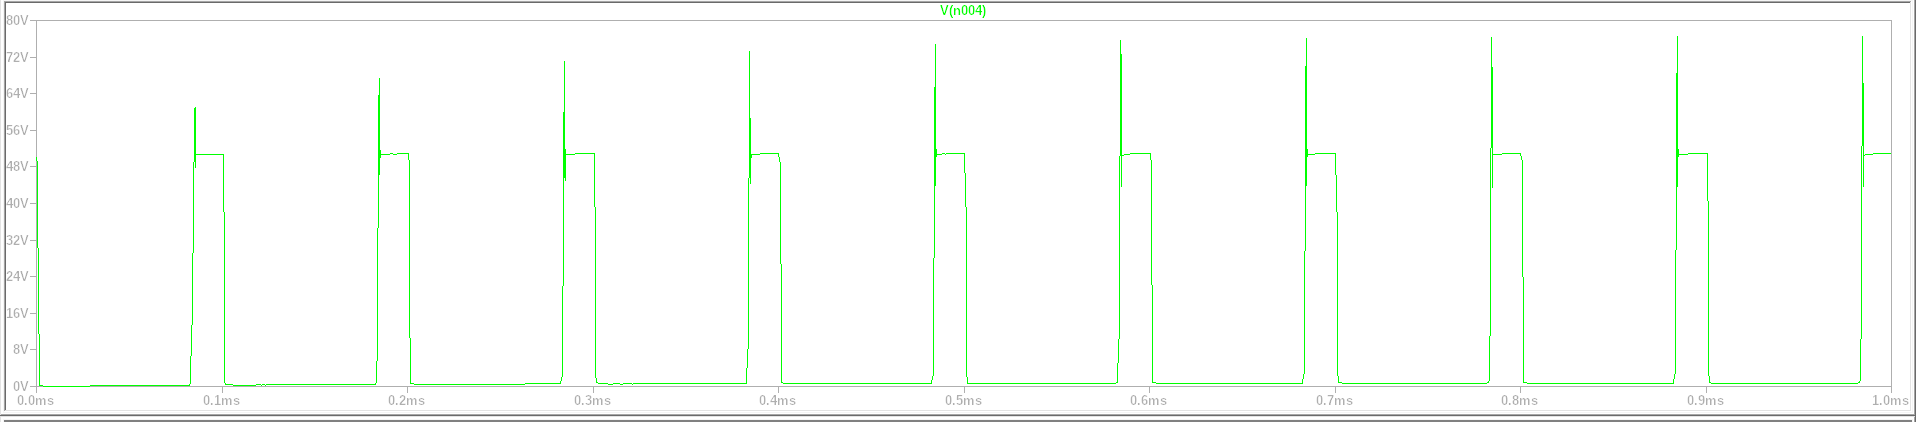
\includegraphics[width=0.8\textwidth]{aun1_rld_with_snubber_rgate100ohm.png}
\caption{Przebieg napiecia na wyjsciu tranzystora MOSFET sterujacego ukladem RLD z rezystancja bramki 100 [Ohm] i z tlumikiem oscylacji D-S}
\end{figure}

\begin{figure}[H]
\centering
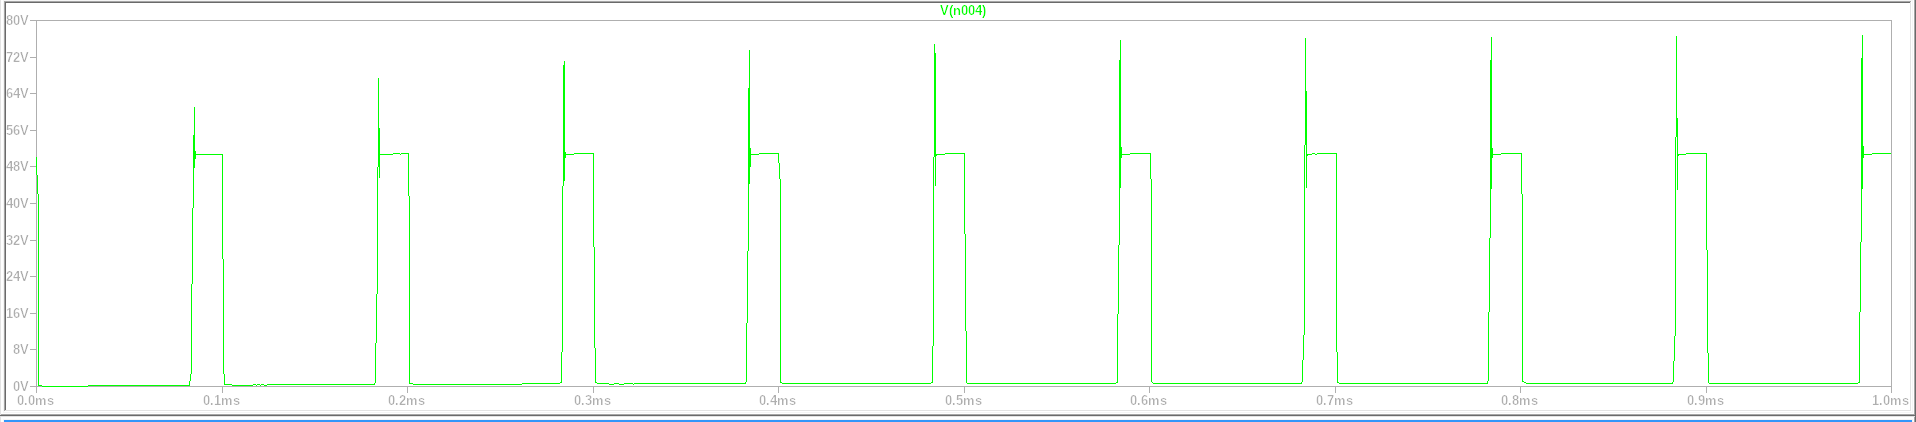
\includegraphics[width=0.8\textwidth]{aun1_rld_with_snubber_rgate10ohm.png}
\caption{Przebieg napiecia na wyjsciu tranzystora MOSFET sterujacego ukladem RLD z rezystancja bramki 10 [Ohm] i z tlumikiem oscylacji D-S}
\end{figure}

\begin{table}[H]
\centering
\begin{tabular}{|l|c|c|}
\hline
\textbf{Tlumik} & \(\mathbf{T_{osc} \ (\mu s)}\) & \(\mathbf{A_{osc} \ (V)}\) \\
\hline
Bez tlumika, \(R_{gate} = 100\,\Omega\) & 1.0958 & 30.7943 \\
\hline
Bez tlumika, \(R_{gate} = 10\,\Omega\) & 1.8058 & 50.8134 \\
\hline
Tlumik, \(R_{gate} = 10\,\Omega\) & 1.0968 & 10.0267 \\
\hline
Tlumik, \(R_{gate} = 100\,\Omega\) & 1.1505 & 10.4941 \\
\hline
\end{tabular}
\caption{Porownanie napiecia na drenie tranzystora MOSFET sterujacym ukladem RLD z oraz bez uzycia tlumika}
\label{tab:oscillation_data}
\end{table}

\end{figure}

\section{Część II}

\subsection{TYPOWA REALIZACJA TORU STEROWANIA TRANZYSTORA MOSFET}

\subsection{MOSTKOWE UKŁADY WZMACZNIACZY TRANZYSTOROWYCH}

\section{Część III}

\subsection{BADANIA EKSPERYMENTALNE}

j) Przebiegi prądów oraz napięć na stanowiskach eksperymentalnych

Uwaga: brak jednostek na osi OY spowodowany jest faktem, ze dane
zapisane byly w formacie raw, niezeskalowane

Przebiegi na stanowisku Alspa- amplituda napiecia 250 [V], amplituda pradu 1.5 [A], regulacja predkosci odbywala sie przez zmiane czestotliwosci napiecia i pradu

\begin{figure}[H]
\centering
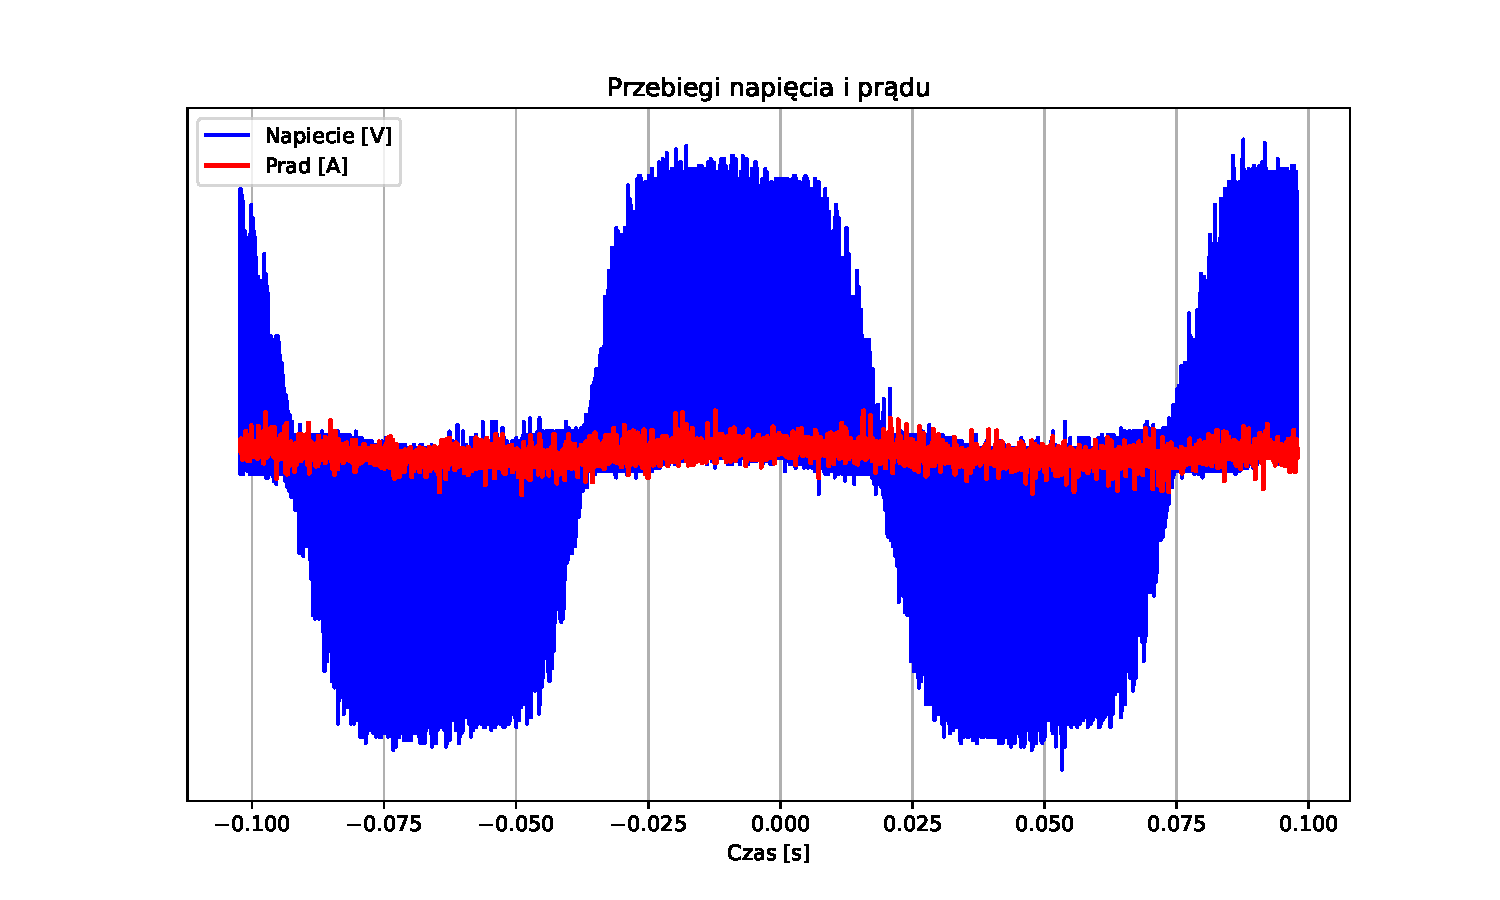
\includegraphics[width=0.8\textwidth]{aun1_alspa_rpm300.pdf}
\caption{Przebieg napiecia oraz pradu na stanowisku Alspa przy predkosci katowej 300 [RPM]}
\end{figure}

\begin{figure}[H]
\centering
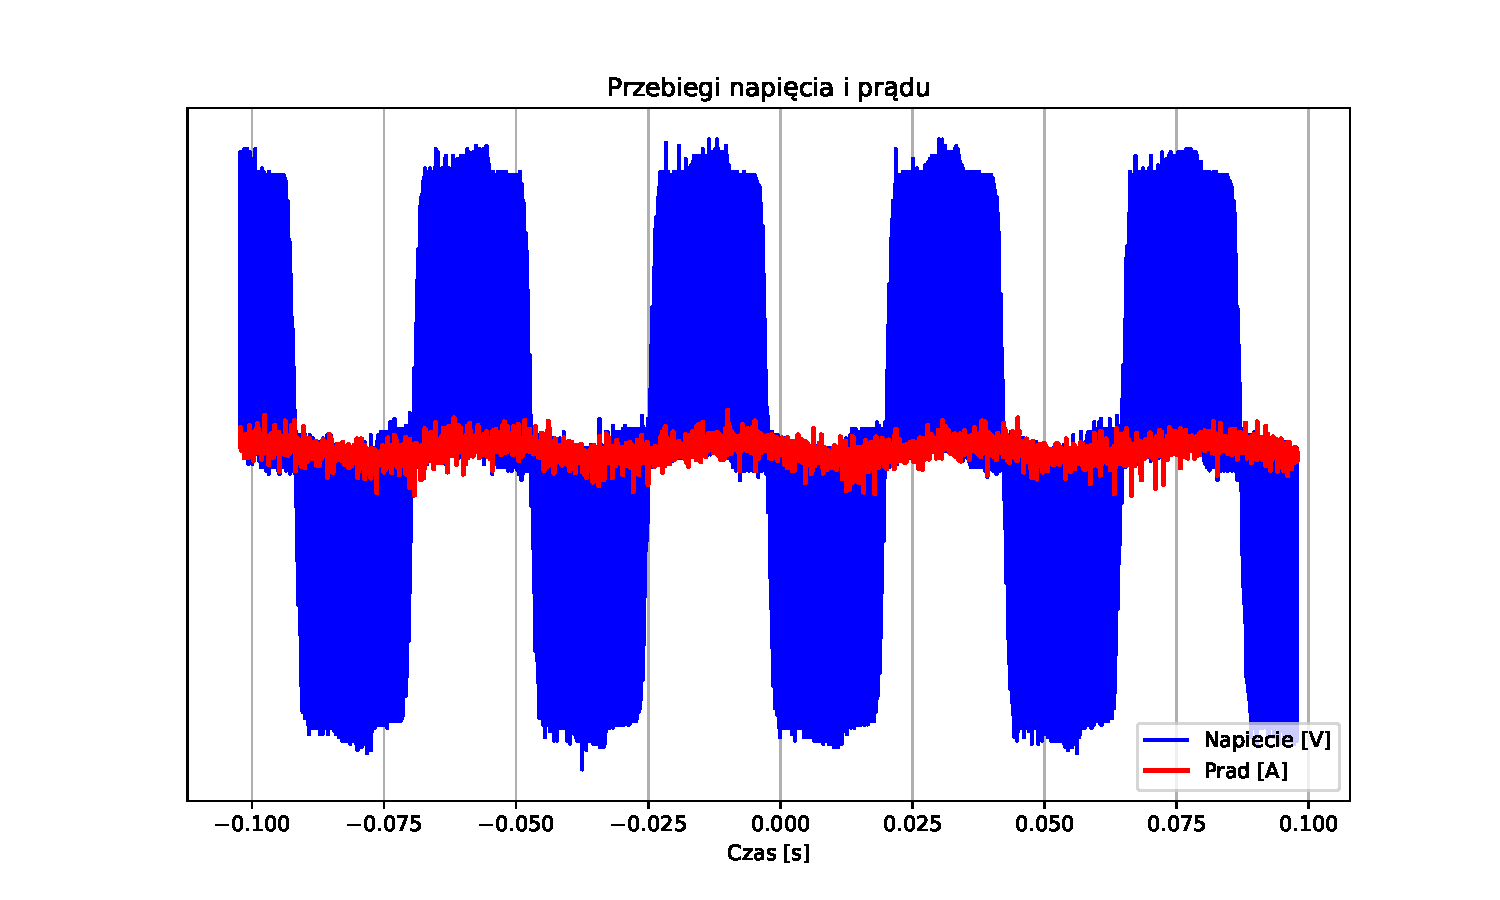
\includegraphics[width=0.8\textwidth]{aun1_alspa_rpm600.pdf}
\caption{Przebieg napiecia oraz pradu na stanowisku Alspa przy predkosci katowej 600 [RPM]}
\end{figure}

\begin{figure}[H]
\centering
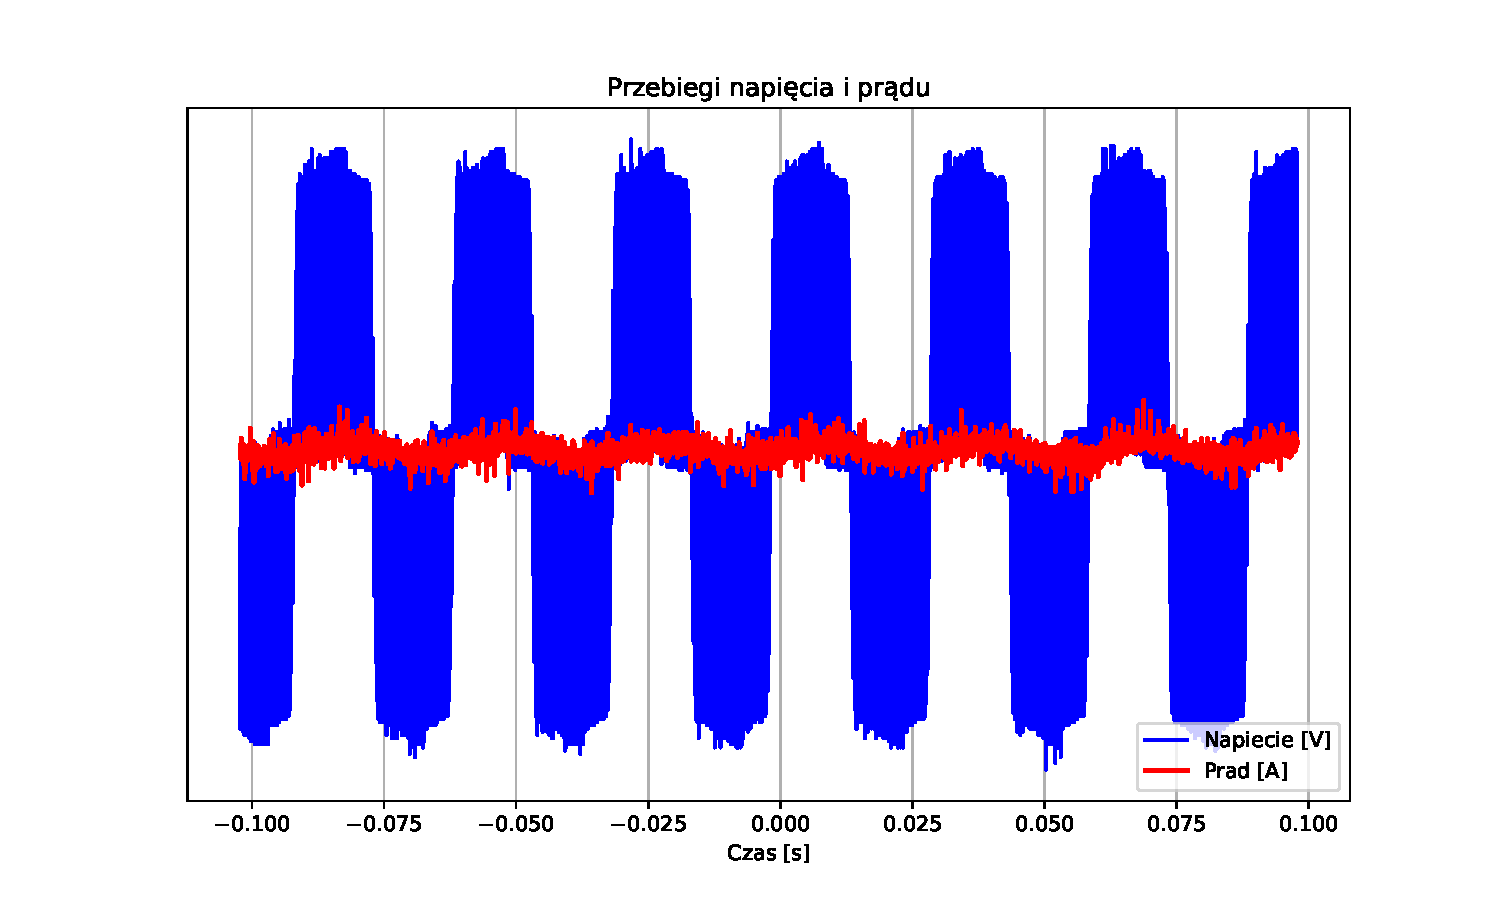
\includegraphics[width=0.8\textwidth]{aun1_alspa_rpm900.pdf}
\caption{Przebieg napiecia oraz pradu na stanowisku Alspa przy predkosci katowej 900 [RPM]}
\end{figure}

Przebiegi na stanowisku Microverter

\begin{figure}[H]
\centering
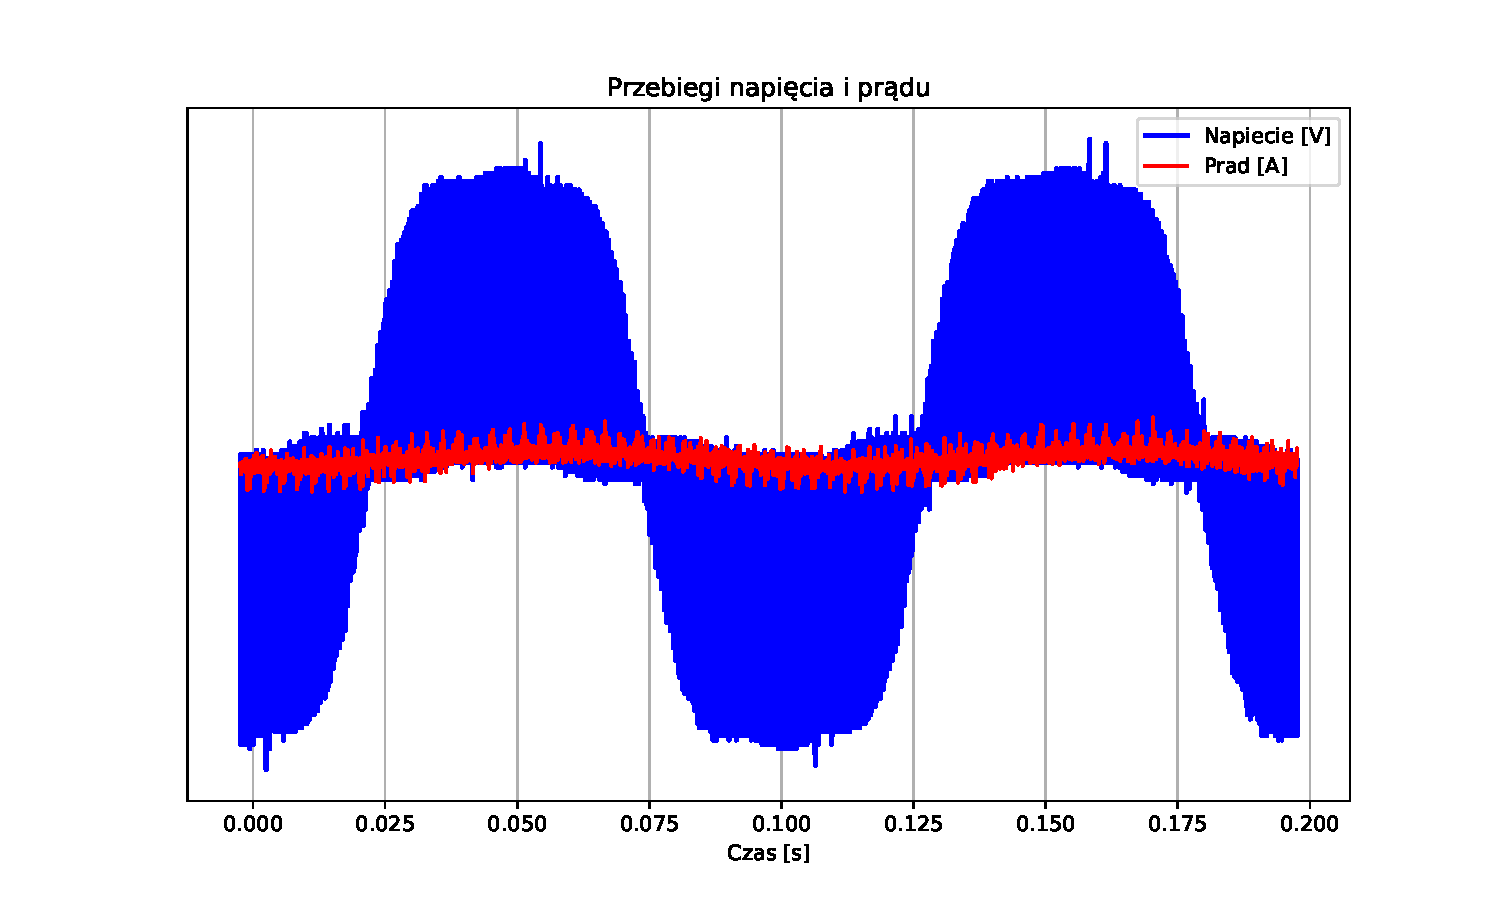
\includegraphics[width=0.8\textwidth]{aun1_microverter_rpm300.pdf}
\caption{Przebieg napiecia oraz pradu na stanowisku Microverter przy predkosci katowej 300 [RPM]}
\end{figure}

\begin{figure}[H]
\centering
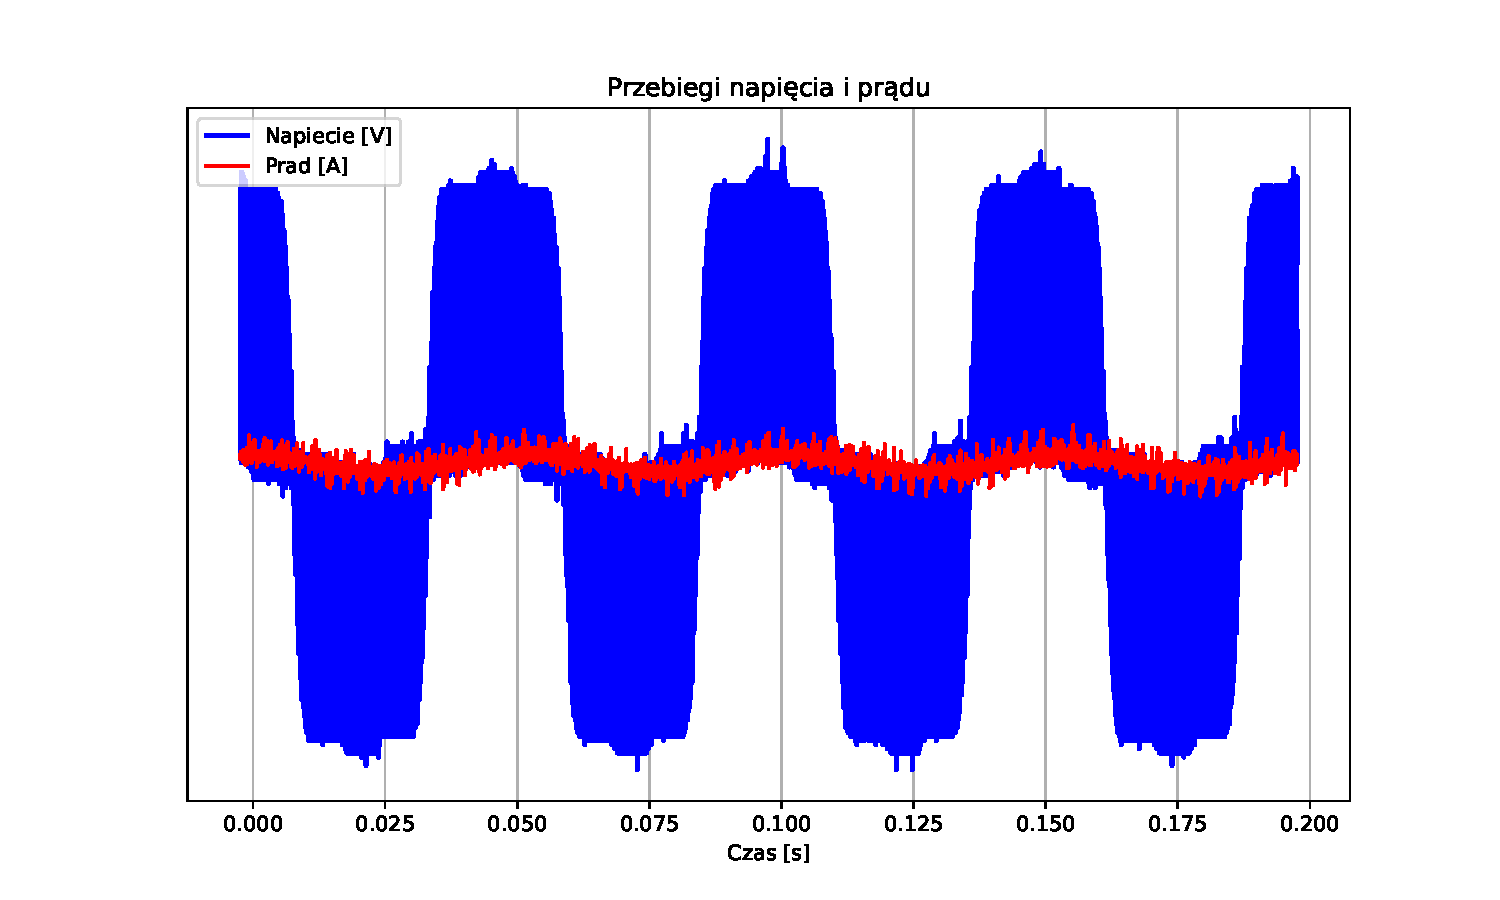
\includegraphics[width=0.8\textwidth]{aun1_microverter_rpm600.pdf}
\caption{Przebieg napiecia oraz pradu na stanowisku Microverter przy predkosci katowej 600 [RPM]}
\end{figure}

\begin{figure}[H]
\centering
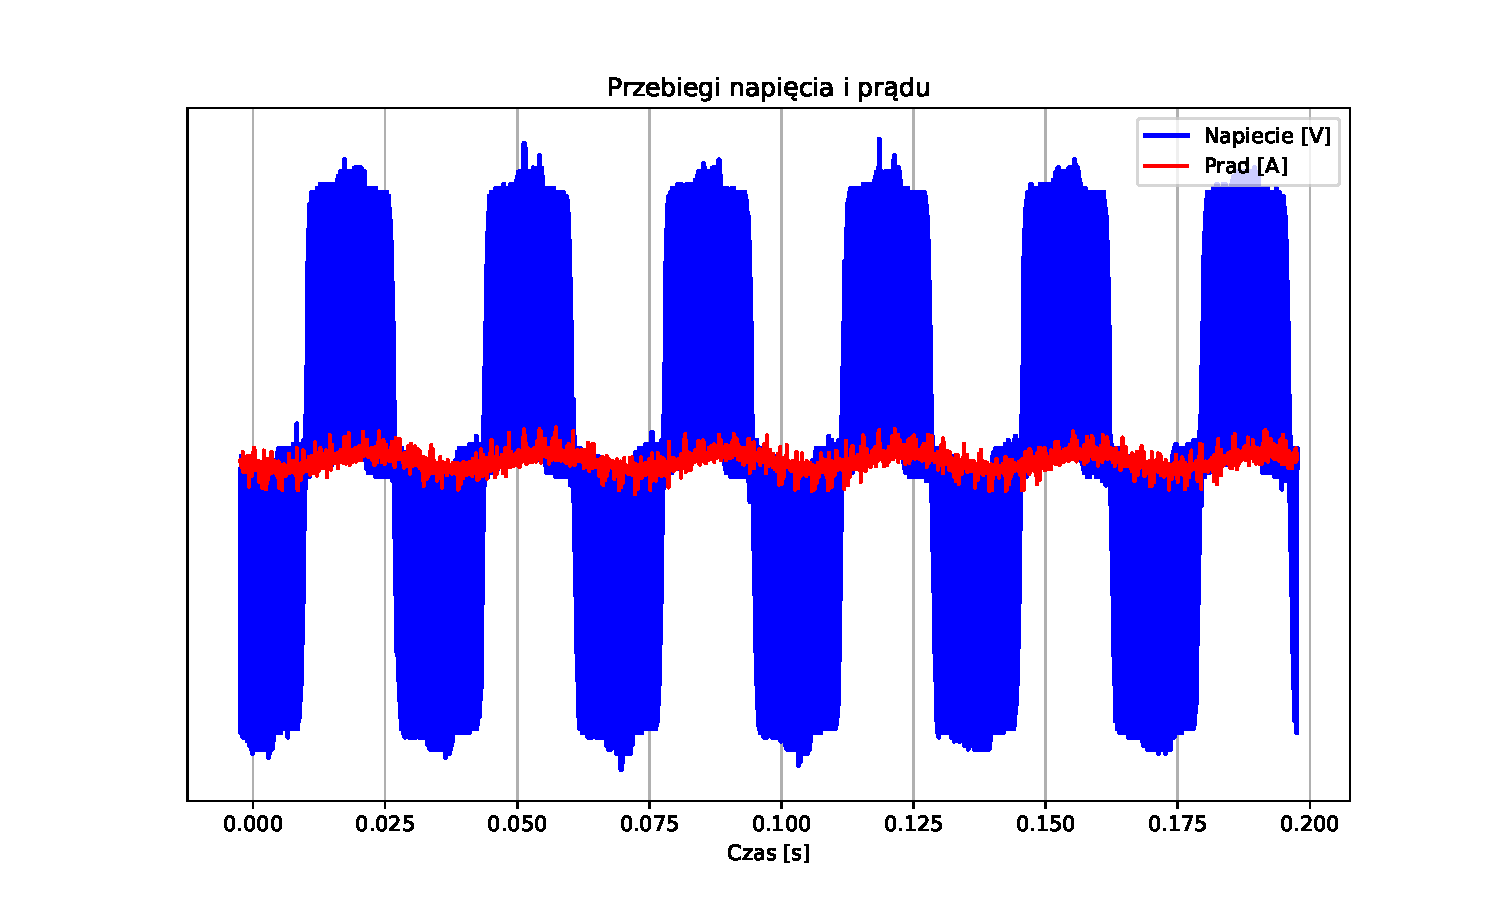
\includegraphics[width=0.8\textwidth]{aun1_microverter_rpm900.pdf}
\caption{Przebieg napiecia oraz pradu na stanowisku Microverter przy predkosci katowej 900 [RPM]}
\end{figure}

Przebiegi napiecia i pradu na stanowisku Unidrive

\begin{figure}[H]
\centering
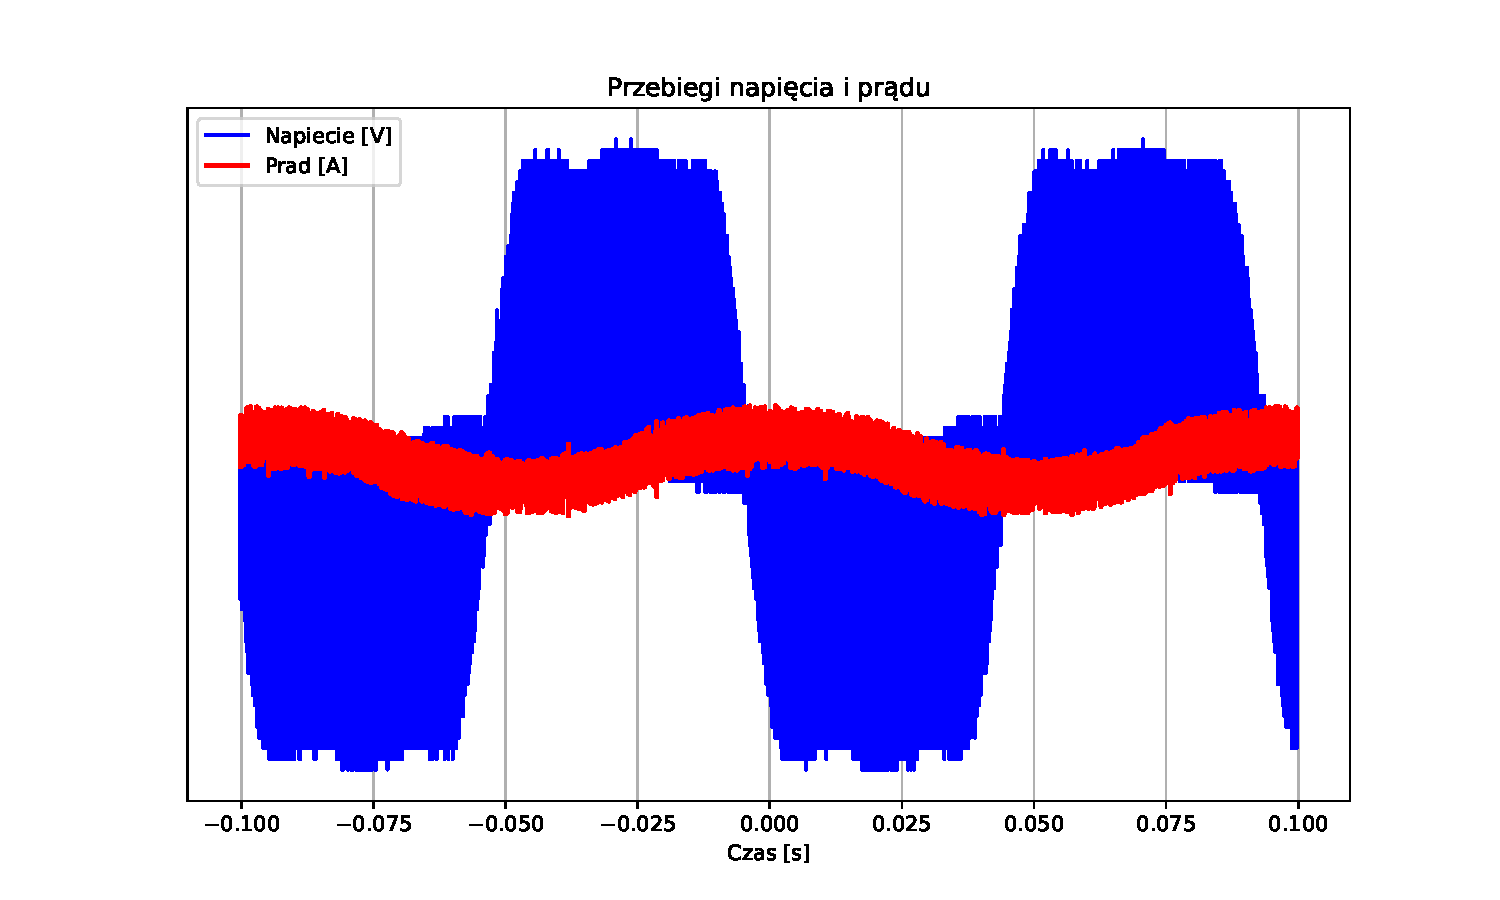
\includegraphics[width=0.8\textwidth]{aun1_unidrive_rpm300.pdf}
\caption{Przebieg napiecia oraz pradu na stanowisku Unidrive przy predkosci katowej 300 [RPM]}
\end{figure}

\begin{figure}[H]
\centering
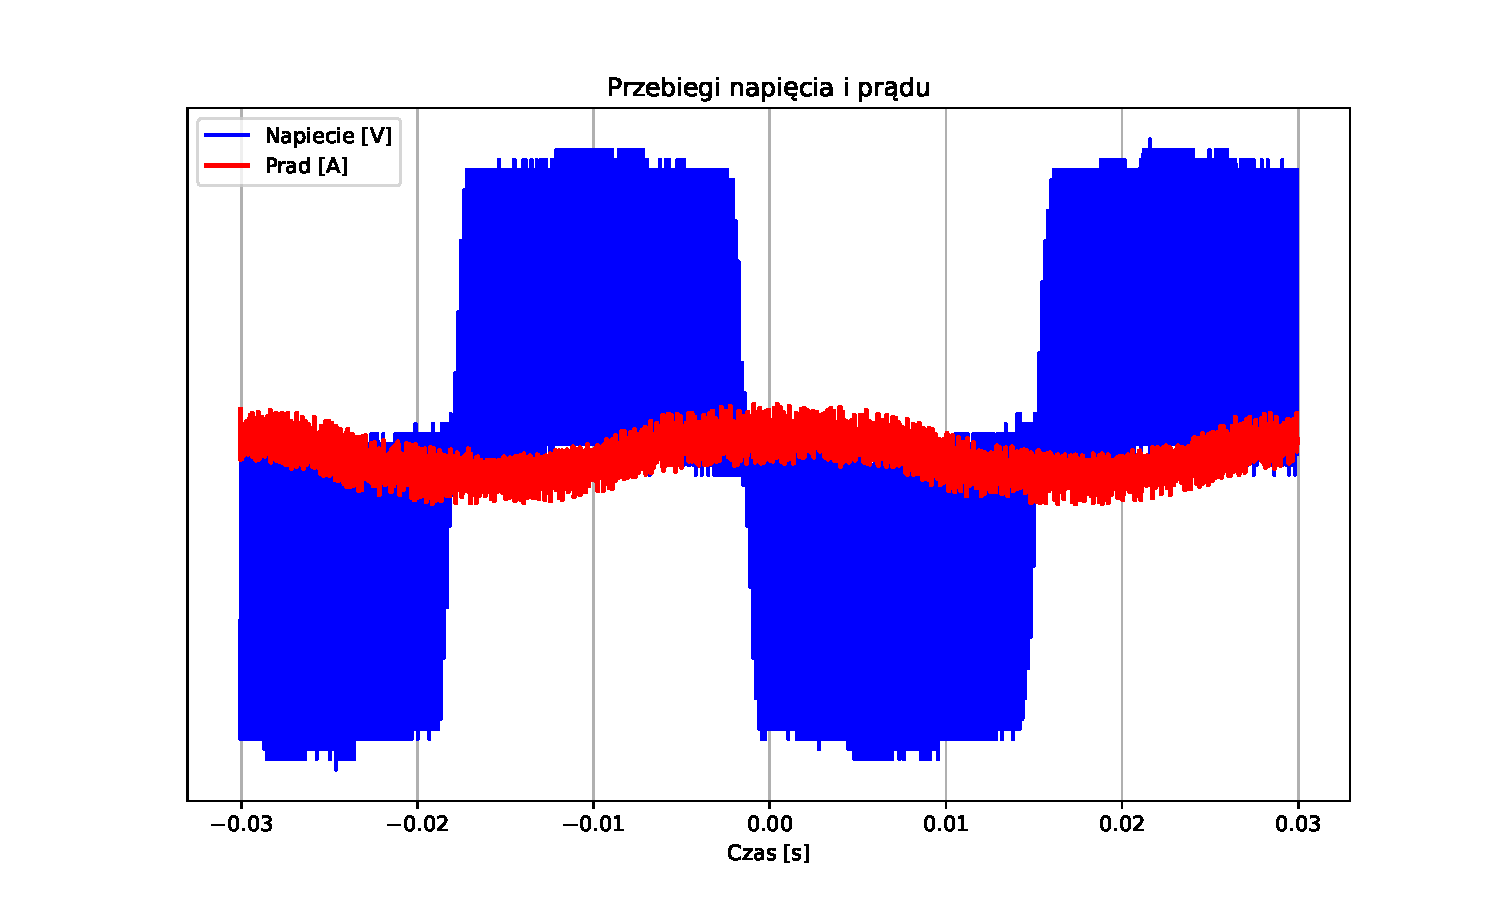
\includegraphics[width=0.8\textwidth]{aun1_unidrive_rpm600.pdf}
\caption{Przebieg napiecia oraz pradu na stanowisku Unidrive przy predkosci katowej 600 [RPM]}
\end{figure}

\begin{figure}[H]
\centering
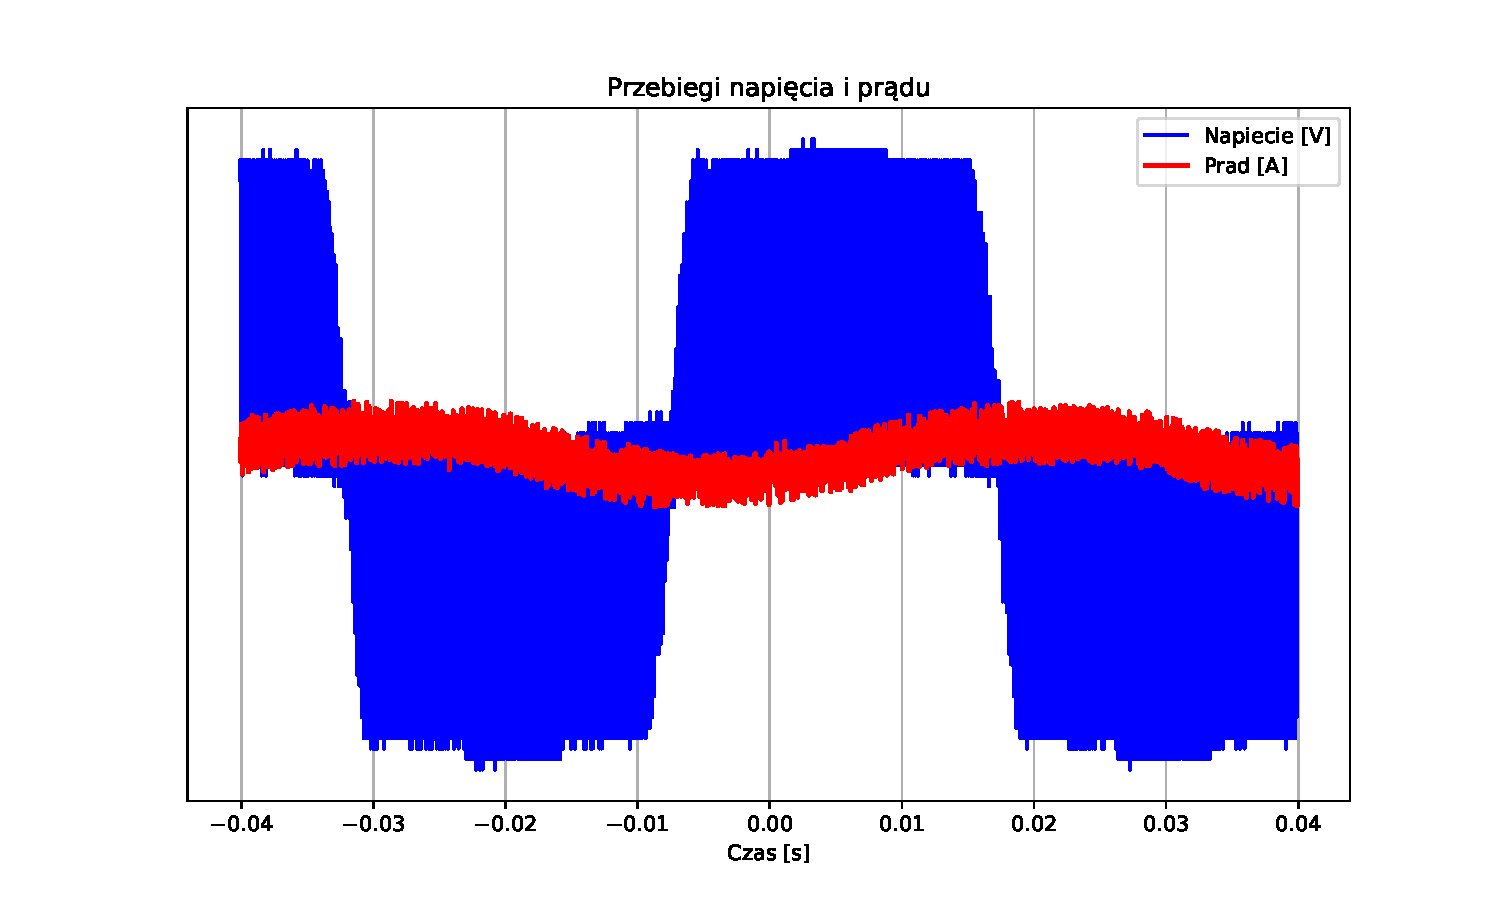
\includegraphics[width=0.8\textwidth]{aun1_unidrive_rpm900.pdf}
\caption{Przebieg napiecia oraz pradu na stanowisku Unidrive przy predkosci katowej 900 [RPM]}
\end{figure}

Przebiegi na stanowisku DML

Uwaga: Niestety, ale grupa od ktorej otrzymalismy te pomiary (prowadzacy zgodzil sie na taki proceder, poniewaz zadna z grup nie zdazyla wykonac eksperymentu na kazdym stanowisku) nie zapisala dla jakich predkosci katowych
byly robione pomiary

\begin{figure}[H]
\centering
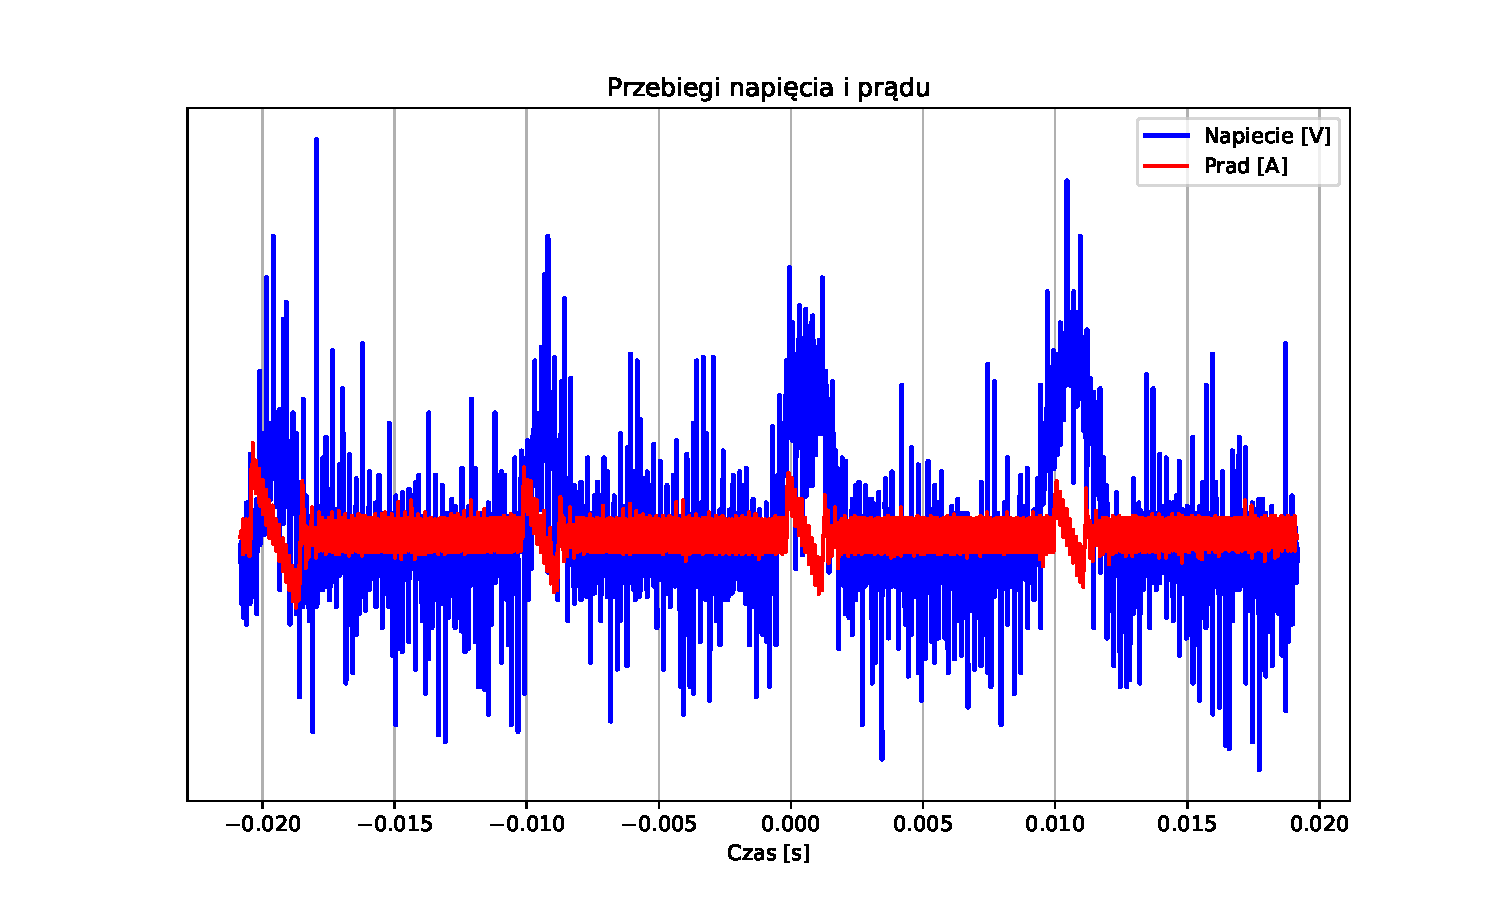
\includegraphics[width=0.8\textwidth]{aun1_dml_obciazenie_weak.pdf}
\caption{Przebieg napiecia oraz pradu na stanowisku Unidrive przy malym obciazeniu}
\end{figure}

\begin{figure}[H]
\centering
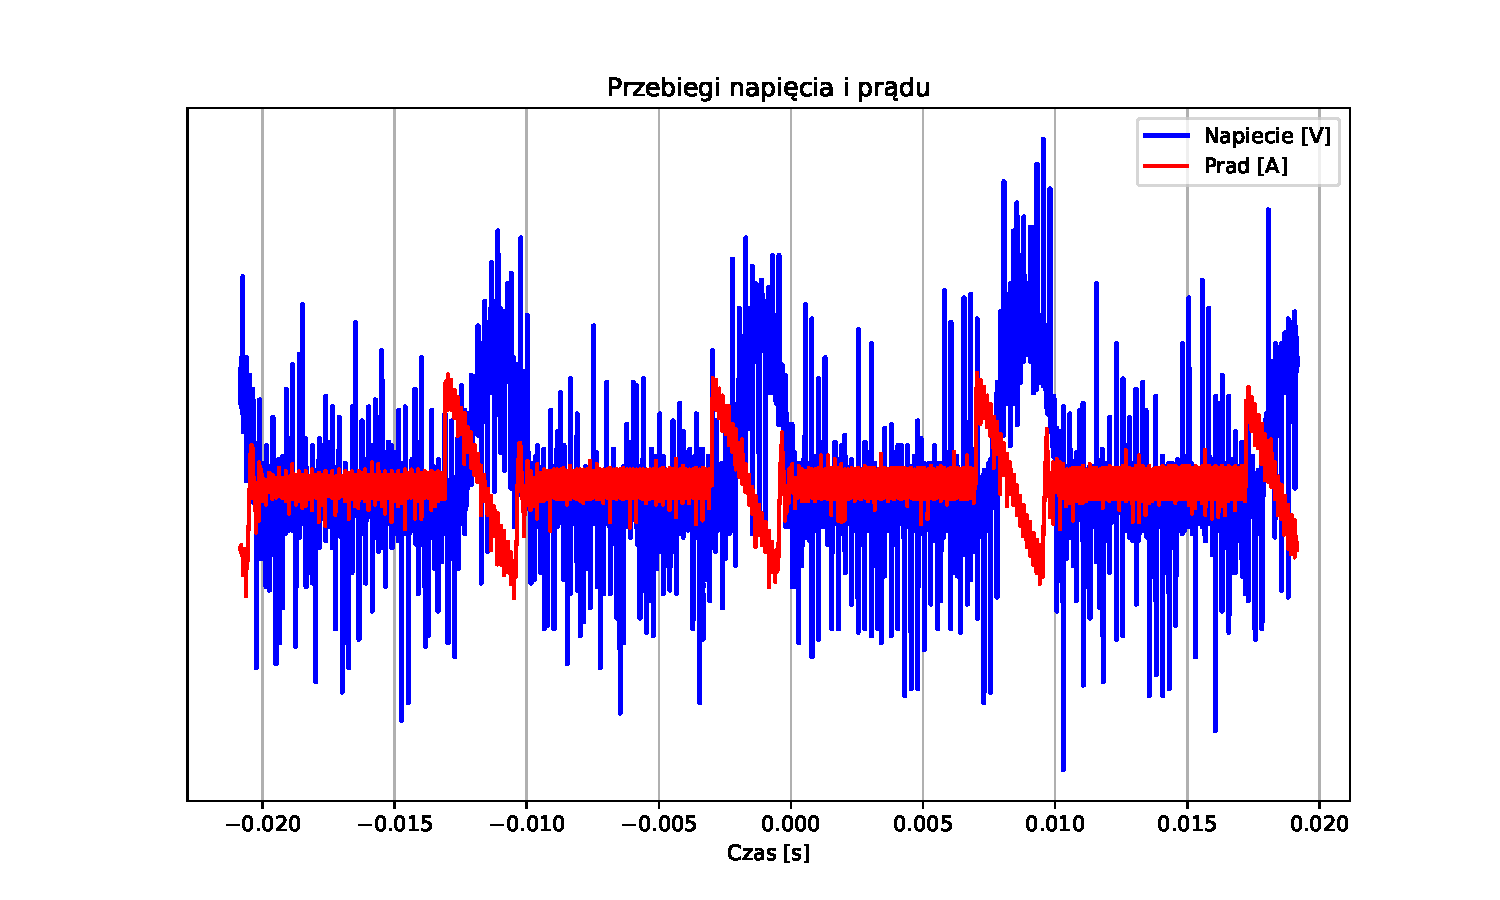
\includegraphics[width=0.8\textwidth]{aun1_dml_obciazenie_medium.pdf}
\caption{Przebieg napiecia oraz pradu na stanowisku Unidrive przy srednim obciazeniu}
\end{figure}

\begin{figure}[H]
\centering
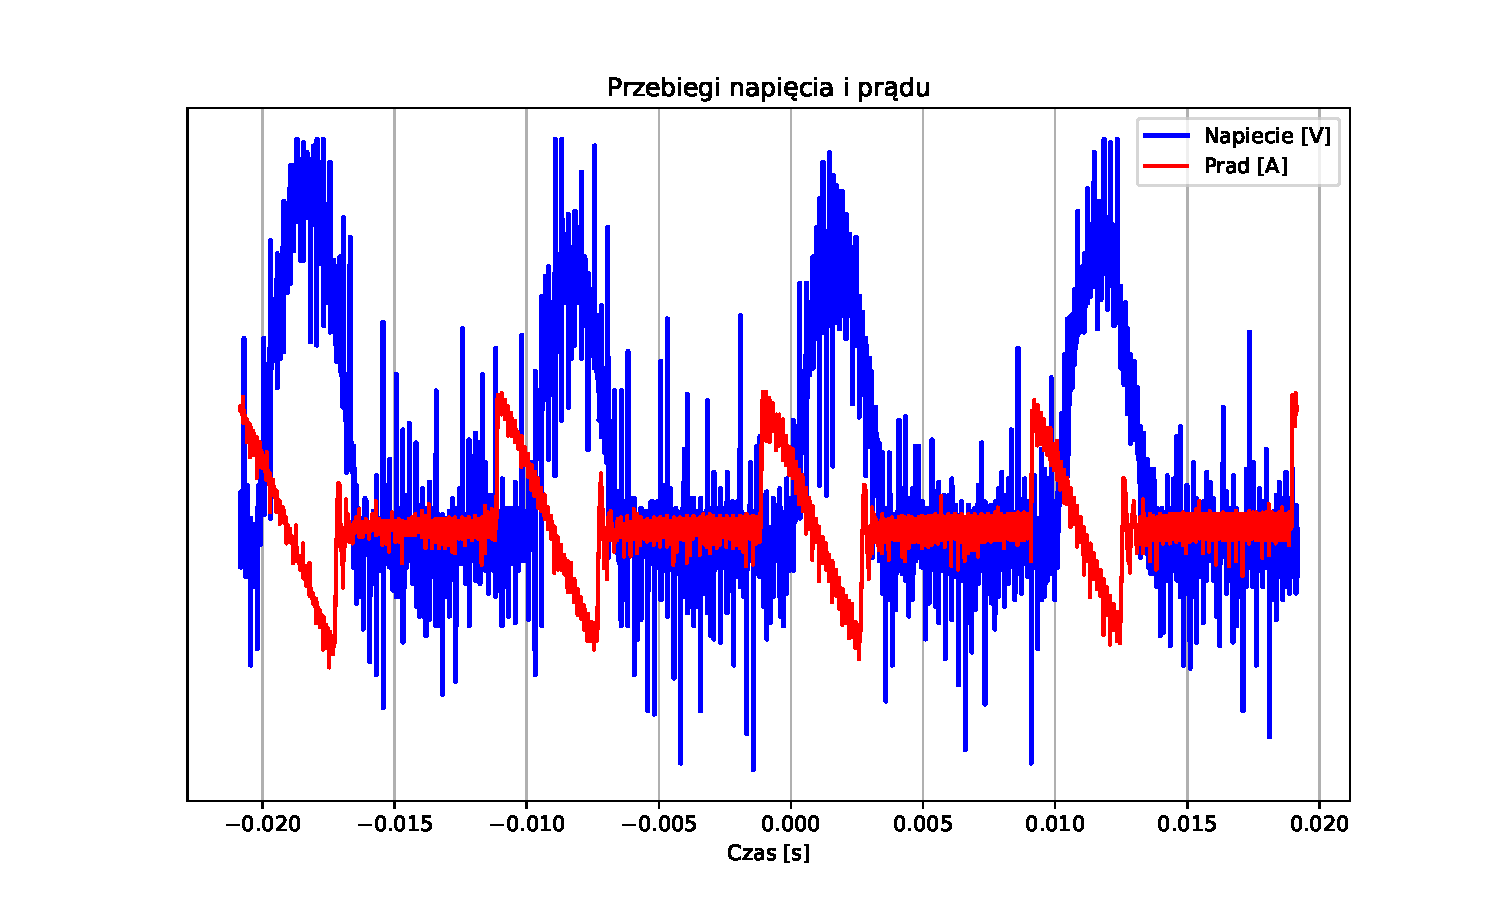
\includegraphics[width=0.8\textwidth]{aun1_dml_obciazenie_hard.pdf}
\caption{Przebieg napiecia oraz pradu na stanowisku Unidrive przy duzym obciazeniu}
\end{figure}


\section{Część IV}

\subsection{MOSTEK TYRYSTOROWY}

\end{document}
